% Options for packages loaded elsewhere
\PassOptionsToPackage{unicode}{hyperref}
\PassOptionsToPackage{hyphens}{url}
%
\documentclass[
  ignorenonframetext,
]{beamer}
\usepackage{pgfpages}
\setbeamertemplate{caption}[numbered]
\setbeamertemplate{caption label separator}{: }
\setbeamercolor{caption name}{fg=normal text.fg}
\beamertemplatenavigationsymbolsempty
% Prevent slide breaks in the middle of a paragraph
\widowpenalties 1 10000
\raggedbottom
\setbeamertemplate{part page}{
  \centering
  \begin{beamercolorbox}[sep=16pt,center]{part title}
    \usebeamerfont{part title}\insertpart\par
  \end{beamercolorbox}
}
\setbeamertemplate{section page}{
  \centering
  \begin{beamercolorbox}[sep=12pt,center]{part title}
    \usebeamerfont{section title}\insertsection\par
  \end{beamercolorbox}
}
\setbeamertemplate{subsection page}{
  \centering
  \begin{beamercolorbox}[sep=8pt,center]{part title}
    \usebeamerfont{subsection title}\insertsubsection\par
  \end{beamercolorbox}
}
\AtBeginPart{
  \frame{\partpage}
}
\AtBeginSection{
  \ifbibliography
  \else
    \frame{\sectionpage}
  \fi
}
\AtBeginSubsection{
  \frame{\subsectionpage}
}

\usepackage{amsmath,amssymb}
\usepackage{iftex}
\ifPDFTeX
  \usepackage[T1]{fontenc}
  \usepackage[utf8]{inputenc}
  \usepackage{textcomp} % provide euro and other symbols
\else % if luatex or xetex
  \usepackage{unicode-math}
  \defaultfontfeatures{Scale=MatchLowercase}
  \defaultfontfeatures[\rmfamily]{Ligatures=TeX,Scale=1}
\fi
\usepackage{lmodern}
\ifPDFTeX\else  
    % xetex/luatex font selection
\fi
% Use upquote if available, for straight quotes in verbatim environments
\IfFileExists{upquote.sty}{\usepackage{upquote}}{}
\IfFileExists{microtype.sty}{% use microtype if available
  \usepackage[]{microtype}
  \UseMicrotypeSet[protrusion]{basicmath} % disable protrusion for tt fonts
}{}
\makeatletter
\@ifundefined{KOMAClassName}{% if non-KOMA class
  \IfFileExists{parskip.sty}{%
    \usepackage{parskip}
  }{% else
    \setlength{\parindent}{0pt}
    \setlength{\parskip}{6pt plus 2pt minus 1pt}}
}{% if KOMA class
  \KOMAoptions{parskip=half}}
\makeatother
\usepackage{xcolor}
\newif\ifbibliography
\setlength{\emergencystretch}{3em} % prevent overfull lines
\setcounter{secnumdepth}{-\maxdimen} % remove section numbering


\providecommand{\tightlist}{%
  \setlength{\itemsep}{0pt}\setlength{\parskip}{0pt}}\usepackage{longtable,booktabs,array}
\usepackage{calc} % for calculating minipage widths
\usepackage{caption}
% Make caption package work with longtable
\makeatletter
\def\fnum@table{\tablename~\thetable}
\makeatother
\usepackage{graphicx}
\makeatletter
\def\maxwidth{\ifdim\Gin@nat@width>\linewidth\linewidth\else\Gin@nat@width\fi}
\def\maxheight{\ifdim\Gin@nat@height>\textheight\textheight\else\Gin@nat@height\fi}
\makeatother
% Scale images if necessary, so that they will not overflow the page
% margins by default, and it is still possible to overwrite the defaults
% using explicit options in \includegraphics[width, height, ...]{}
\setkeys{Gin}{width=\maxwidth,height=\maxheight,keepaspectratio}
% Set default figure placement to htbp
\makeatletter
\def\fps@figure{htbp}
\makeatother

\makeatletter
\@ifpackageloaded{caption}{}{\usepackage{caption}}
\AtBeginDocument{%
\ifdefined\contentsname
  \renewcommand*\contentsname{Table of contents}
\else
  \newcommand\contentsname{Table of contents}
\fi
\ifdefined\listfigurename
  \renewcommand*\listfigurename{List of Figures}
\else
  \newcommand\listfigurename{List of Figures}
\fi
\ifdefined\listtablename
  \renewcommand*\listtablename{List of Tables}
\else
  \newcommand\listtablename{List of Tables}
\fi
\ifdefined\figurename
  \renewcommand*\figurename{Figure}
\else
  \newcommand\figurename{Figure}
\fi
\ifdefined\tablename
  \renewcommand*\tablename{Table}
\else
  \newcommand\tablename{Table}
\fi
}
\@ifpackageloaded{float}{}{\usepackage{float}}
\floatstyle{ruled}
\@ifundefined{c@chapter}{\newfloat{codelisting}{h}{lop}}{\newfloat{codelisting}{h}{lop}[chapter]}
\floatname{codelisting}{Listing}
\newcommand*\listoflistings{\listof{codelisting}{List of Listings}}
\makeatother
\makeatletter
\makeatother
\makeatletter
\@ifpackageloaded{caption}{}{\usepackage{caption}}
\@ifpackageloaded{subcaption}{}{\usepackage{subcaption}}
\makeatother

\ifLuaTeX
  \usepackage{selnolig}  % disable illegal ligatures
\fi
\usepackage{bookmark}

\IfFileExists{xurl.sty}{\usepackage{xurl}}{} % add URL line breaks if available
\urlstyle{same} % disable monospaced font for URLs
\hypersetup{
  pdftitle={Gains from Asset Trade},
  pdfauthor={I Made Krisna Gupta},
  hidelinks,
  pdfcreator={LaTeX via pandoc}}


\title{Gains from Asset Trade}
\subtitle{ECES905205 pertemuan 6}
\author{I Made Krisna Gupta}
\date{October 3, 2024}

\begin{document}
\frame{\titlepage}


\begin{frame}{Intro}
\phantomsection\label{intro}
\begin{itemize}
\item
  In this chapter, we see how financially open economies can, in theory,
  reap gains from financial globalization in the long run.
\item
  We first look at the factors that limit international borrowing and
  lending, then we look at how a nation's ability to use international
  financial markets allows it to accomplish three different goals:

  \begin{itemize}
  \tightlist
  \item
    Consumption smoothing (by steadying consumption when income
    fluctuates)
  \item
    Efficient investment (by borrowing to build a productive capital
    stock)
  \item
    Diversification of risk (by trading of stocks between countries)
  \end{itemize}
\end{itemize}
\end{frame}

\begin{frame}{Borrowing constraint}
\phantomsection\label{borrowing-constraint}
\begin{itemize}
\tightlist
\item
  The ability to borrow in times of need and lend in times of prosperity
  has profound effects on a country's well-being.
\item
  Using changes in an economy's external wealth, we can derive the key
  constraint that limits its borrowing in the long run: the long-run
  budget constraint (LRBC).
\item
  The LRBC tells us precisely how and why a country must, in the long
  run, ``live within its means.''
\end{itemize}
\end{frame}

\begin{frame}{Borrowing constraint}
\phantomsection\label{borrowing-constraint-1}
When a household borrows \$100,000 at 10\% annually, there are two
different ways it can deal with its debt each year:

\begin{itemize}
\tightlist
\item
  Case 1 A debt that is serviced. You pay the interest but you never pay
  any principal.
\item
  Case 2 A debt that is not serviced. You pay neither interest nor
  principal. Your debt grows by 10\% each year.
\end{itemize}

Case 2 is not sustainable. Sometimes called a rollover scheme, a pyramid
scheme, or a Ponzi game, this case illustrates the limits on the use of
borrowing.

In the long run, lenders will not allow the debt to grow larger. This is
the essence of the long-run budget constraint.
\end{frame}

\begin{frame}{Long-run budget constraint}
\phantomsection\label{long-run-budget-constraint}
Here are some assumptions we make in the model economy:

\begin{itemize}
\item
  The country is a small open economy: The country is a price taker and
  cannot influence prices in world markets for goods and services, nor
  can it influence the real interest rate.
\item
  It is a real economy: Prices are perfectly flexible. Analysis is in
  terms of real variables, and we ignore monetary aspects of the
  economy. There is one real good and one real asset.
\item
  The asset, real debt, carries a real interest rate \(r^*\), the world
  real interest rate, which is constant. The country can lend or borrow
  an unlimited amount at this interest rate.
\end{itemize}
\end{frame}

\begin{frame}{Long-run budget constraint}
\phantomsection\label{long-run-budget-constraint-1}
\begin{itemize}
\item
  The country pays a real interest rate \(r^*\) on its start-of-period
  debt liabilities L and is also paid r* on its start-of-period debt
  assets A. Net interest income payments equal to \(r^*A − r^*L\), or
  \(r^*W\), where W is external wealth \((A − L)\).
\item
  There are no unilateral transfers (NUT = 0), no capital transfers (KA
  = 0), and no capital gains on external wealth. Therefore, there are
  only two nonzero items in the current account: the trade balance TB
  and net factor income from abroad, \(r^*W\).
\end{itemize}
\end{frame}

\begin{frame}{Long-run budget constraint}
\phantomsection\label{long-run-budget-constraint-2}
Change in external wealth from end of \(N-1\) to end of \(N\) is given
by:

\[
\Delta W_N=\underbrace{W_N-W_{N-1}}_{\text{Change in external wealth}}=TB_N+\underbrace{r^*W_{N-1}}_{\text{interest paid/received}}
\]

Wealth at the end of the year thus:

\[
W_N=TB_N+(1+r^*)W_{N-1}
\]
\end{frame}

\begin{frame}{LR budget constraint}
\phantomsection\label{lr-budget-constraint}
At the end of year 0: \(W_0=(1+r^*)W_{-1}+TB_0\)

We assume that all debts owed or owing must be paid off, and the country
must end that year with zero external wealth.

At the end of year 1: \(W_1=0=(1+r^*)W_0+TB_1\)

Cobined: \(W_1=0=(1+r^*)^2W_{-1}+(1+r^*)TB_0+TB_1\)

2 period budget constraint become:

\[
-(1+r^*)^2W_{-1}=(1+r^*)TB_0+TB_1
\]
\end{frame}

\begin{frame}{LR budget constraint}
\phantomsection\label{lr-budget-constraint-1}
Divide our previous equation with \((1+r^*)\), we get:

\[
\underbrace{-(1+r^*)W_{-1}}_{\text{Minus last period wealth PV}}=\underbrace{TB_0+\frac{TB_1}{(1+r^*)}}_{\text{PV of trade balances}}
\]

The present value of X in period N is the amount that would have to be
set aside now so that, with accumulated interest, \(X\) is available in
\(N\) periods. If the interest rate is \(r^*\), then the present value
of \(X\) is \(X/(1 + r^*)^N\).
\end{frame}

\begin{frame}{LRBC}
\phantomsection\label{lrbc}
Let \(N\) go to infinity, we get infinite sum and arriveat LRBC:

\[
-(1+r^*)W_{-1}=TB_0+\frac{TB_1}{(1+r^*)}+\frac{TB_2}{(1+r^*)^2}+\cdots
\] A debtor (creditor) country must have future trade balances that are
offsetting and positive (negative) in present value terms.
\end{frame}

\begin{frame}{Perpetual Loan}
\phantomsection\label{perpetual-loan}
Let's compute \(PV(X)\) for any stream of constant payment starting in
period 1:

\[
\frac{X}{(1+r^*)}+\frac{X}{(1+r^*)^2}+\frac{X}{(1+r^*)^3}+\cdots=\frac{X}{r^*}
\]

For example, the PV of such a stream of payments of a perpetual loan,
with \(X=100\) and \(r^*=0.05\) equals:

\[
\frac{100}{(1+5\%)}+\frac{100}{(1+5\%)^2}+\frac{100}{(1+5\%)^3}+\cdots=\frac{X}{5\%}=2,000
\]
\end{frame}

\begin{frame}{LRBC}
\phantomsection\label{lrbc-1}
\begin{itemize}
\tightlist
\item
  Since TB=GDP-GNE, LRBC says that \emph{in present value terms, a
  country's expenditures (GNE) must equal its production (GDP) plus any
  initial wealth}.
\end{itemize}

\[
(1+r^*)W_{-1}+GDP_0+\frac{GDP_1}{(1+r^*)}+\frac{GDP_2}{(1+r^*)^2}+\cdots \\
=GNE_0+\frac{GNE_1}{(1+r^*)}+\frac{GNE_2}{(1+r^*)^2}+\cdots
\]

Present value of present and future GNE = present value of country's
spending.
\end{frame}

\begin{frame}{Exorbitant privilege}
\phantomsection\label{exorbitant-privilege}
The US has been a net debtr with \(W=A-L<0\) since the 1980s. Negative
external wealth leads to a deficit n net factor income from abroad with
\(r^*W=r^*(A-L)<0\). Yet as we saw yesterweek, US net factor income from
abroad has been positive throughout this period.

\begin{itemize}
\item
  The only way a net debtor can earn a positive net interest income is
  by receiving a higher rate of interest on its assets than it pays on
  its liabilities.
\item
  e.g., in the 1960s French officials complained that the US has the
  ``exorbitant privilege'' of being able to borrow cheaply while earning
  higher returns on its foreign investments.
\end{itemize}
\end{frame}

\begin{frame}{Manna from Heaven}
\phantomsection\label{manna-from-heaven}
\begin{itemize}
\item
  The United States enjoys positive capital gains, KG, on its external
  wealth. These large capital gains on external assets and the smaller
  capital losses on external liabilities are gains that cannot be
  otherwise measured, so their accuracy and meaning is controversial.
\item
  Some skeptics call these capital gains ``statistical manna from
  heaven.''
\item
  Others think these gains are real and may reflect the United States
  acting as a kind of ``venture capitalist to the world.''
\item
  As with the ``exorbitant privilege,'' this financial gain for the
  United States is a loss for the rest of the world.
\end{itemize}
\end{frame}

\begin{frame}{US privilege}
\phantomsection\label{us-privilege}
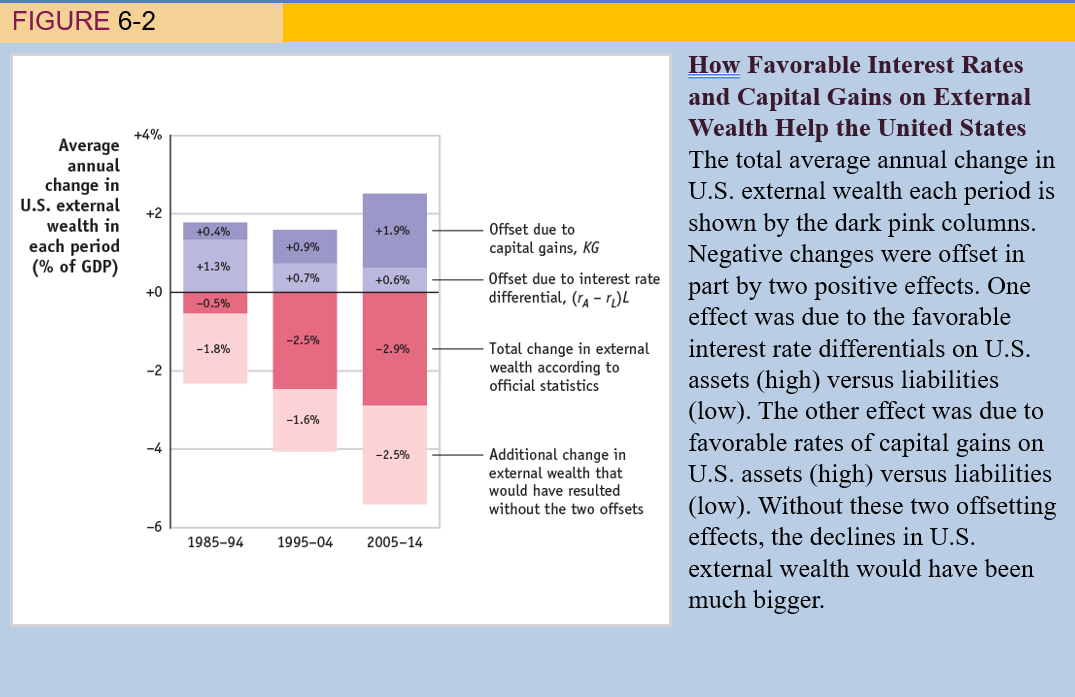
\includegraphics{pic1.png}
\end{frame}

\begin{frame}{Conclusion}
\phantomsection\label{conclusion}
When we add the +1.5\% capital gain differential to the +0.5\% interest
differential, we end up with a US total return differential
(interest+capital gains) of about 2\% per year since the 1980s. For
comparison, in the same period, the total return differential was close
to zero in every other G7 country.

\[
\Delta W_N=W_N-W_{N-1}=TB_N+r^*W_{N-1}+(r^*-r^0)L+KG
\]
\end{frame}

\begin{frame}{Emerging market}
\phantomsection\label{emerging-market}
The US borrows low and lends high. For most poorer countries, the
opposite is true. They borrow high and lend low. This is because they
are riskier borrowers and lenders.

Because of country risk, investors typically demand a risk premium
before they will invest in any assets issued by these countries, whether
government debt, private equity, private debt, or FDI.
\end{frame}

\begin{frame}{Close vs Open}
\phantomsection\label{close-vs-open}
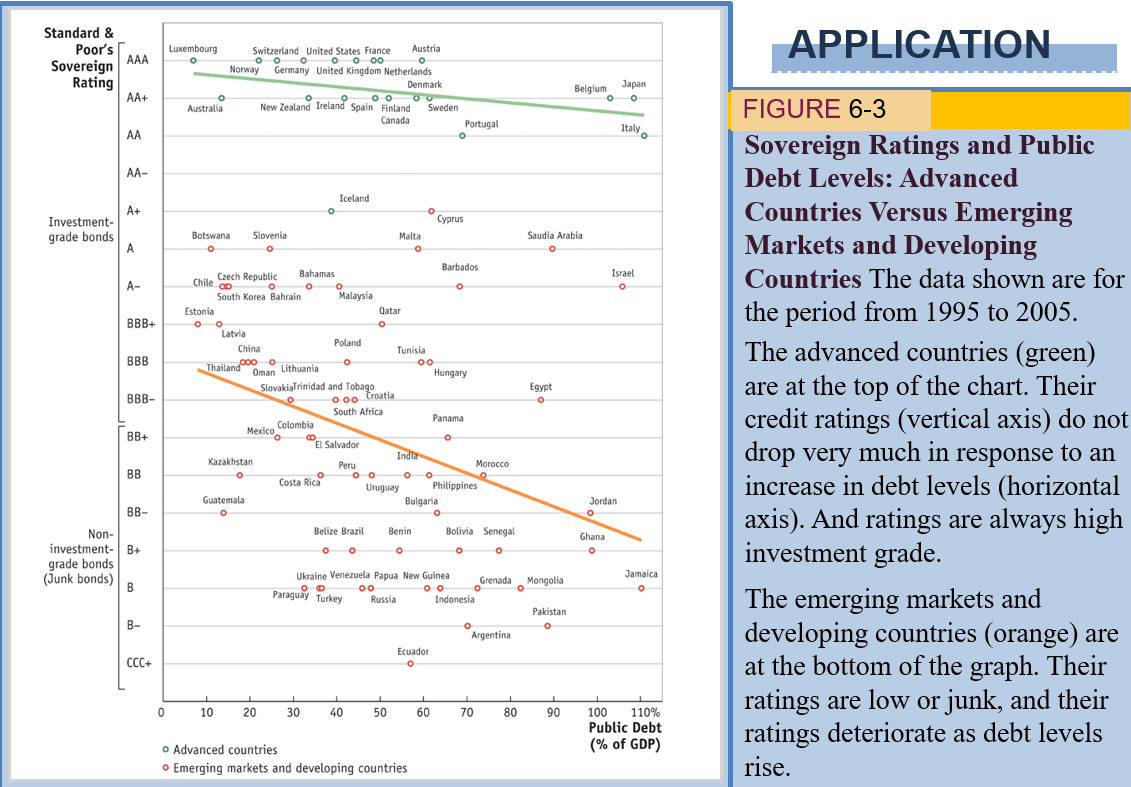
\includegraphics{pic2.png}
\end{frame}

\begin{frame}{Consumption smoothing}
\phantomsection\label{consumption-smoothing}
In this section, we use the long-run budget constraint and a simplified
model of an economy to examine the gains from financial globalization.

We focus on the gains that result when an open economy uses external
borrowing and lending to eliminate an important kind of risk, namely,
undesirable fluctuations in aggregate consumption.
\end{frame}

\begin{frame}{Consumption smoothing}
\phantomsection\label{consumption-smoothing-1}
We now examine the gains from external borrowing and lending, allowing
an economy to eliminate fluctuations in aggregate consumption. We adopt
some additional assumptions:

\begin{itemize}
\item
  Real output or GDP (denoted Q) is produced using labor as the only
  input. Production of GDP may be subject to shocks; depending on the
  shock, the same amount of labor input may yield different amounts of
  output.
\item
  We use the terms ``household'' and ``country'' interchangeably.
  Preferences of the country/household are such that it will choose a
  level of consumption C that is constant over time. This level of
  smooth consumption must be consistent with the LRBC.
\end{itemize}
\end{frame}

\begin{frame}{Consumption smoothing}
\phantomsection\label{consumption-smoothing-2}
\begin{itemize}
\item
  For now, we assume consumption is the only source of demand. Both
  investment I and government spending G are zero; therefore, GNE equals
  personal consumption expenditures C.
\item
  Our analysis begins at time 0, and we assume the country begins with
  zero initial wealth inherited from the past, so that W−1 is equal to
  zero.
\item
  We assume that the country is small and the rest of the world (ROW) is
  large, and the prevailing world real interest rate is constant at
  \(r^*\). In the numerical examples that follow, we will assume
  \(r* = 0.05 = 5\%\) per year.
\end{itemize}
\end{frame}

\begin{frame}{Consumption smoothing}
\phantomsection\label{consumption-smoothing-3}
These assumptions give us a special case of the LRBC that requires the
present value of current and future trade balances to equal zero (amid
zero initial wealth):

\[
\underbrace{0}_{\text{initial W}}=\text{PV of TB}=\underbrace{\text{PV of } Q}_{PV \  GDP}-\underbrace{\text{PV of } C}_{PV \ GNE}
\]
\end{frame}

\begin{frame}{Close vs Open}
\phantomsection\label{close-vs-open-1}
In a closed economy, TB will always be zero, trhus LRBC will always be
satisifed. There won't be any gains from financial globalization. Under
no shock, the same thing is true. No need to do anything.

\begin{longtable}[]{@{}llllllll@{}}
\toprule\noalign{}
period & 0 & 1 & 2 & 3 & 4 & \ldots{} & \(r^*=0.05\) \\
\midrule\noalign{}
\endhead
GDP Q & 100 & 100 & 100 & 100 & 100 & \ldots{} & 2,100 \\
GNE C & 100 & 100 & 100 & 100 & 100 & \ldots{} & 2,100 \\
TB & 0 & 0 & 0 & 0 & 0 & 0 & 0 \\
\bottomrule\noalign{}
\end{longtable}
\end{frame}

\begin{frame}{Close vs Open}
\phantomsection\label{close-vs-open-2}
Suppose there's unanticipted -21 shock in year 0 then returns to Q=100
after that. with \(r^*=5\%\), PV reduces by 1\%. With no trade of asset,
the reduction of GDP equate exactly with GDP, because in a closed
economy, TB=0.

\begin{longtable}[]{@{}llllllll@{}}
\toprule\noalign{}
period & 0 & 1 & 2 & 3 & 4 & \ldots{} & \(r^*=0.05\) \\
\midrule\noalign{}
\endhead
GDP Q & 79 & 100 & 100 & 100 & 100 & \ldots{} & 2,079 \\
GNE C & 79 & 100 & 100 & 100 & 100 & \ldots{} & 2,079 \\
TB & 0 & 0 & 0 & 0 & 0 & 0 & 0 \\
\bottomrule\noalign{}
\end{longtable}
\end{frame}

\begin{frame}{Close vs Open}
\phantomsection\label{close-vs-open-3}
However, under open economy regime, consumption can be smoothen while
still satisfying LRBC by reducing consumption by 1\% for each year. The
present value of C is then: 99 + 99/0.05 = 2,079. PV GDP = PV GNE.

\begin{longtable}[]{@{}llllllll@{}}
\toprule\noalign{}
period & 0 & 1 & 2 & 3 & 4 & \ldots{} & \(r^*=0.05\) \\
\midrule\noalign{}
\endhead
GDP Q & 79 & 100 & 100 & 100 & 100 & \ldots{} & 2,079 \\
GNE C & 99 & 99 & 99 & 99 & 99 & \ldots{} & 2,079 \\
TB & -20 & +1 & +1 & +1 & +1 & \ldots{} & 0 \\
NFIA & 0 & -1 & -1 & -1 & -1 & \ldots{} & - \\
CA & -20 & 0 & 0 & 0 & 0 & \ldots{} & - \\
W & -20 & -20 & -20 & -20 & -20 & \ldots{} & - \\
\bottomrule\noalign{}
\end{longtable}
\end{frame}

\begin{frame}{Generalizing}
\phantomsection\label{generalizing}
\begin{itemize}
\tightlist
\item
  Suppose, more generally, that output \(Q\) and consumption \(C\) are
  initially stable at some value with \(Q = C\) and external wealth of
  zero. The LRBC is satisfied.
\item
  If output falls in year 0 by ΔQ and then returns to its prior value
  for all future periods, then the present value of output decreases by
  ΔQ.
\item
  To meet the LRBC, a closed economy lowers its consumption by the whole
  ΔQ in year 0.
\item
  An open economy can lower its consumption uniformly (every period) by
  a smaller amount so that ΔC \textless{} ΔQ.
\end{itemize}
\end{frame}

\begin{frame}{Consumption smoothing}
\phantomsection\label{consumption-smoothing-4}
\begin{itemize}
\item
  A loan of \(\Delta Q-\Delta C\) in year 0 requires interest payment of
  \(r^*(\Delta Q -\Delta C)\) in later years.
\item
  In future years consumption cuts create trade surpluses of
  \(\Delta C\), and if these are to cover the interst paymets, then
  \(\Delta C\) must be chosen so that
\end{itemize}

\[
r^*(\Delta Q-\Delta C)=\Delta C
\] where \(\Delta Q- \Delta C\) is the amount borrowed in year 0.
Rearranging above, we get

\[
\Delta C=\frac{r^*}{1+r^*} \Delta Q
\]
\end{frame}

\begin{frame}{Permanent shock}
\phantomsection\label{permanent-shock}
With a permanent shock, output will be lower by ΔQ in all years, so the
only way either a closed or open economy can satisfy the LRBC while
keeping consumption smooth is to cut consumption by ΔC = ΔQ in all
years.

Comparing the results for a temporary shock and a permanent shock, we
see an important point:

\begin{itemize}
\item
  Consumers can smooth out temporary shocks---they have to adjust a bit.
  But the adjustment is far smaller than the shock itself---yet they
  must
\item
  adjust immediately and fully to permanent shocks.
\end{itemize}
\end{frame}

\begin{frame}{Gains from smoothing}
\phantomsection\label{gains-from-smoothing}
Financial openness allows countries to ``save for a rainy day.'' Without
financial institutions, you have to spend what you earn each period.

\begin{itemize}
\tightlist
\item
  Using financial transactions to smooth consumption fluctuations makes
  a household and/or country better off.
\item
  In a closed economy, Q = C, so output fluctuations immediately
  generate consumption fluctuations.
\item
  In an open economy, the desired smooth consumption path can be
  achieved by running a trade deficit during bad times and a trade
  surplus during good times.
\end{itemize}
\end{frame}

\begin{frame}{C and financial openness}
\phantomsection\label{c-and-financial-openness}
\begin{itemize}
\item
  Does the evidence show that countries avoid consumption volatility by
  embracing financial globalization?
\item
  The ratio of a country's consumption to the volatility of its output
  should fall as more consumption smoothing is achieved.
\item
  In our model of a small, open economy that can borrow or lend without
  limit, this ratio should fall to zero when the gains from financial
  globalization are realized.
\end{itemize}

-Since not all shocks are global, countries ought to be able to achieve
some reduction in consumption volatility through external finance.
\end{frame}

\begin{frame}{Some evidence}
\phantomsection\label{some-evidence}
\begin{figure}[H]

{\centering 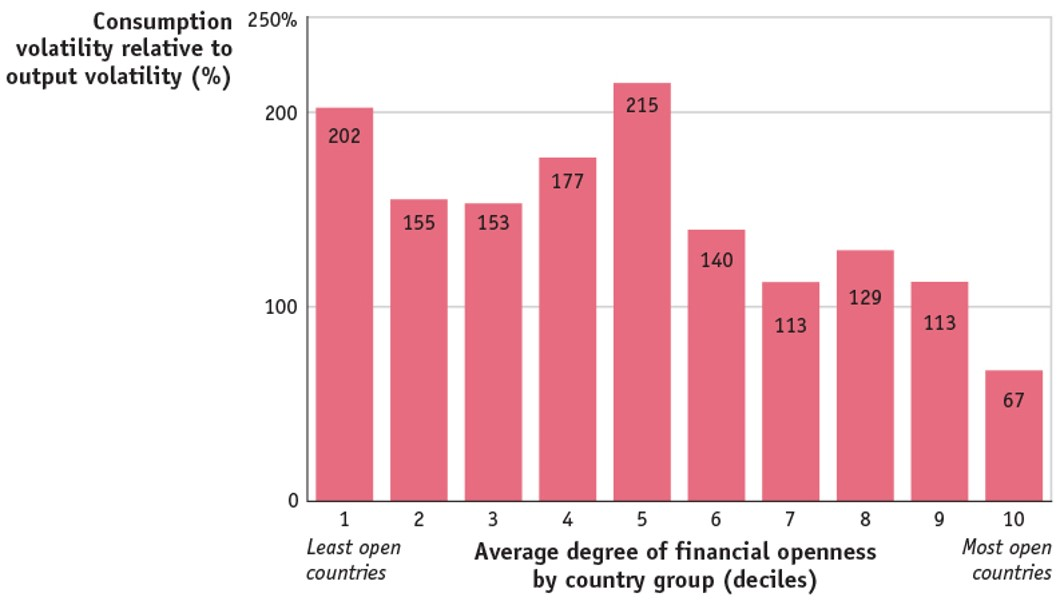
\includegraphics{Picture1.jpg}

}

\caption{Feenstra \& Taylor compute consumption volatility/output
volatility of 166 countriesfrom 1990-2010, then arrange them from least
open to most open. \textless100\%=not volatile. Apparently even in a
relatively open countries, (desile 8), ratio still exceed 100\%}

\end{figure}%
\end{frame}

\begin{frame}{Remarks}
\phantomsection\label{remarks}
The lack of evidence suggests that some of the relatively high
consumption volatility must be unrelated to financial openness.

Consumption-smoothing gains in emerging markets require improving poor
governance and weak institutions, developing their financial systems,
and pursuing further financial liberalization.
\end{frame}

\begin{frame}{Sovereign Wealth Funds}
\phantomsection\label{sovereign-wealth-funds}
\begin{itemize}
\item
  Countries may engage in precautionary saving, whereby the government
  acquires a buffer of external assets, a ``rainy day'' fund.
\item
  Precautionary saving is on the rise and takes two forms. The first is
  the accumulation of foreign reserves by central banks, which may be
  used to achieve certain goals, such as maintaining a fixed exchange
  rate, or as reserves that can be deployed during a sudden stop.
\item
  The second form is called sovereign wealth funds, whereby state-owned
  asset management companies invest some of the government savings.
\end{itemize}
\end{frame}

\begin{frame}{SWF}
\phantomsection\label{swf}
\begin{itemize}
\item
  During a three-year copper boom, Chile set aside \$48.6 billion, more
  than 30 percent of the country's gross domestic product, resisting
  calls for more government spending.
\item
  At the time, the finance minister Andrés Velasco was criticized for
  austerity, but after the global credit freeze in 2008, Chile unveiled
  a \$4 billion package of tax cuts and subsidies, including aid to poor
  families.
\item
  ``People finally understood what was behind his `stinginess' of early
  years,'' said Sebastian Edwards, a Chilean economist at the University
  of California, Los Angeles.
\end{itemize}
\end{frame}

\begin{frame}{Efficient investment}
\phantomsection\label{efficient-investment}
\begin{itemize}
\item
  Openness may also deliver gains by improving a country's ability to
  augment its capital stock and take advantage of new production
  opportunities.
\item
  Assume that producing output requires labor and capital, which is
  created over time by investing output.
\item
  When we make this change, the LRBC must be modified to include
  investment I as a component of GNE. We still assume that government
  consumption G is zero.
\item
  With this change, the LRBC becomes \(0=\text{PV for TB}\)
\end{itemize}
\end{frame}

\begin{frame}{Efficient investment}
\phantomsection\label{efficient-investment-1}
Since PV of TB is the difference between PV of Q and C,

\[
\text{PV of Q}=\text{PV of C}+\text{PV of I}
\]

\begin{itemize}
\item
  A closed economy, in which external borrowing and lending are not
  possible, the trade balance is zero in all periods, and the LRBC is
  automatically satisfied.
\item
  An open economy, in which borrowing and lending are possible, the
  trade balance can be more or less than zero, and we must verify that
  the LRBC is
\end{itemize}
\end{frame}

\begin{frame}{Efficient investment}
\phantomsection\label{efficient-investment-2}
Baseline case, no investment: Q=100, C=100, I=0, TB=0. W=0

\begin{itemize}
\item
  Now assume a shock in year 0 in the form of a new investment
  opportunity: requires an expenditure of 16 units, and will pay off in
  future years by increasing the country's output by 5 units in year 1
  and all subsequent years (but not in year 0).
\item
  Output would be 100 today, then 105 in every subsequent year.
\item
  The present value of this stream of output is 100 plus 105/0.05 or
  2,200, and the present value of consumption must equal 2,200 minus 16,
  or 2,184.
\end{itemize}
\end{frame}

\begin{frame}{Efficient investment}
\phantomsection\label{efficient-investment-3}
\begin{longtable}[]{@{}llllllll@{}}
\toprule\noalign{}
period & 0 & 1 & 2 & 3 & 4 & \ldots{} & \(r^*=0.05\) \\
\midrule\noalign{}
\endhead
GDP Q & 100 & 105 & 105 & 105 & 105 & \ldots{} & 2,079 \\
GNE C & 104 & 104 & 104 & 104 & 104 & \ldots{} & 2,079 \\
GNE I & 16 & 0 & 0 & 0 & 0 & \ldots{} & 16 \\
TB & -20 & +1 & +1 & +1 & +1 & \ldots{} & 0 \\
NFIA & 0 & -1 & -1 & -1 & -1 & \ldots{} & - \\
CA & -20 & 0 & 0 & 0 & 0 & \ldots{} & - \\
W & -20 & -20 & -20 & -20 & -20 & \ldots{} & - \\
\bottomrule\noalign{}
\end{longtable}

The economy run a deficit TB to invest, then surplus to pay em back.
\end{frame}

\begin{frame}{Generalizing}
\phantomsection\label{generalizing-1}
\begin{itemize}
\tightlist
\item
  Suppose that a country starts with zero external wealth, constant
  output Q, consumption C equal to output, and investment I equal to
  zero.
\item
  An investment opportunity appears requiring ΔK units of output in year
  0. This investment will generate an additional ΔQ units of output in
  year 1 and all later years (but not in year 0).
\end{itemize}

\[
\Delta PVQ=\frac{\Delta Q}{(1+r^*)}+\frac{\Delta Q}{(1+r^*)^2}+\frac{\Delta Q}{(1+r^*)^3}+\cdots=\frac{\Delta Q}{r^*}
\]

\begin{itemize}
\tightlist
\item
  Investment will increase the PV of C in and only if
  \(\Delta Q/r^* \geq \Delta K\)
\end{itemize}
\end{frame}

\begin{frame}{Efficient investment}
\phantomsection\label{efficient-investment-4}
The change in \(PV(I)\) is simply \(\Delta K\). Investment will increase
the PV of consumption if and only if \(\Delta Q/r^* \geq \Delta K\).
Rearranging:

\[
\Delta Q \geq r^* \times \Delta K
\]

Dividing by \(\Delta K\), investment is undertaken when

\[
\frac{\Delta Q}{\Delta K} \geq r^*
\]

Firms will invest in projects as long as the marginal product of
capital, or MPK, is at least as great as the real interest rate.
\end{frame}

\begin{frame}{Efficient investment}
\phantomsection\label{efficient-investment-5}
\begin{itemize}
\item
  In an open economy, firms borrow and repay to undertake investment
  that maximizes the present value of output.
\item
  When investing, an open economy sets its MPK equal to the world real
  rate of interest.
\item
  In a closed economy, any resources invested are not consumed. More
  investment implies less consumption. This creates a trade-off.
\item
  Financial openness helps countries to ``make hay while the sun
  shines'' without having to engage in a trade-off against the important
  objective of consumption smoothing.
\end{itemize}
\end{frame}

\begin{frame}{Norway case}
\phantomsection\label{norway-case}
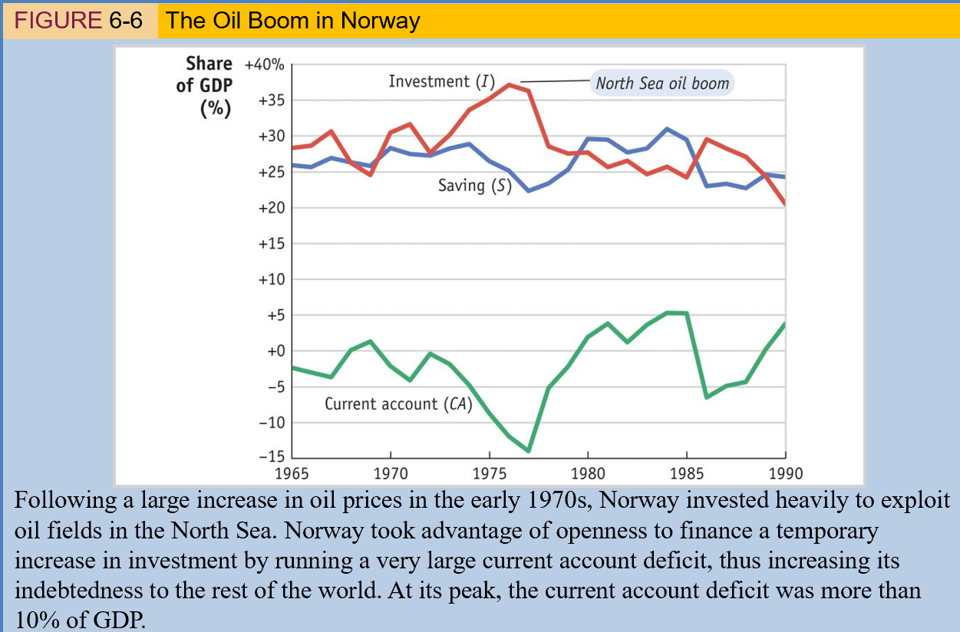
\includegraphics{Picture2.png}
\end{frame}

\begin{frame}{Can poor country gain?}
\phantomsection\label{can-poor-country-gain}
If the world real interest rate is r* and a country has investment
projects for which MPK exceeds r*, then the country should borrow to
finance those projects. With this in mind, we ask: Why doesn't more
capital flow to poor countries?

To look at what determines a country's marginal product of capital,
economists use a version of a production function that maps available
capital per worker, k = K/L, and the prevailing level of productivity A
to the level of output per worker, q = Q/L, where Q is GDP.
\end{frame}

\begin{frame}{Production fn approach}
\phantomsection\label{production-fn-approach}
\[
\underbrace{q}_{\text{Output per worker}}=\underbrace{A}_{\text{productivity level}} \times \underbrace{k^\theta}_{\text{Capital per worker}}
\]

where \(\theta\) is a number between 0 and 1 that measures the
contribution of capital to production, or the elasticity of capital with
respect to output. θ is estimated to be 1/3, and setting the
productivity level at 1, we have:

\[
q=k^{1/3}
\]

MPK, the slope of the production function is given by

\[
MPK=\frac{\Delta q}{\Delta k}=\theta Ak^{\theta-1}=\theta \times \frac{q}{k}
\]
\end{frame}

\begin{frame}{efficient investment}
\phantomsection\label{efficient-investment-6}
\begin{itemize}
\tightlist
\item
  Assuming countries have the same level of productivity, A = 1, our
  model implies that the poorer the country, the higher its MPK, due to
  the assumptions of diminishing marginal product and a common
  productivity level.
\item
  Investment ought to be very profitable in Mexico (and India, and all
  poor countries).
\item
  Investment in Mexico should continue until rates of return are
  equalized. This trajectory is called convergence.
\item
  If the world is characterized by convergence, countries can reach the
  level of capital per worker and output per worker of the rich country
  through investment and capital accumulation.
\end{itemize}
\end{frame}

\begin{frame}
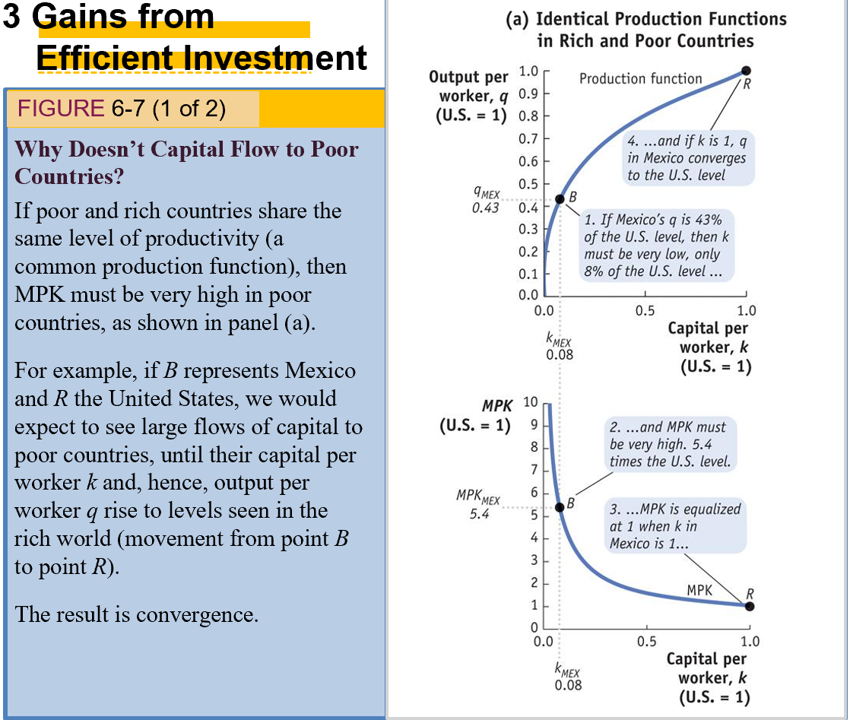
\includegraphics{Picture3.png}
\end{frame}

\begin{frame}
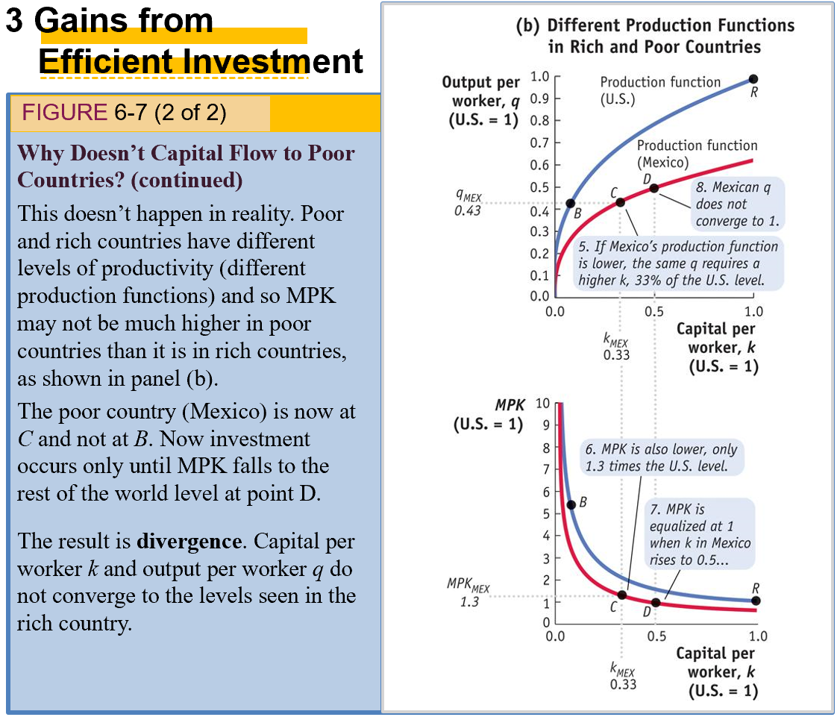
\includegraphics{Picture4.png}
\end{frame}

\begin{frame}{Lucas paradox}
\phantomsection\label{lucas-paradox}
In his widely cited article ``Why Doesn't Capital Flow from Rich to Poor
Countries?'' Nobel laureate Robert Lucas wrote:

\begin{quote}
If this model were anywhere close to being accurate, and if world
capital markets were anywhere close to being free and complete, it is
clear that, in the face of return differentials of this magnitude,
investment goods would flow rapidly from the United States and other
wealthy countries to India and other poor countries. Indeed, one would
expect no investment to occur in the wealthy countries. . . .
\end{quote}
\end{frame}

\begin{frame}{Efficient investment}
\phantomsection\label{efficient-investment-7}
To see why capital does not flow to poor countries, we now suppose that
A, the productivity level, is different in the United States and Mexico,
as denoted by country subscripts. Then:

\[
q_{US}=A_{US}k^{\theta}_{US} \ \ \ \ \ \ \ \ \ \ \ q_{US}=A_{MX}k^{\theta}_{MX} \\
\frac{MPK_{MX}}{MPK_{US}}=\frac{\theta \ q_{MX}}{\theta q_{US}/k_{US}}=\frac{q_{MX}/q_{US}}{k_{MX}/k_{US}}
\]
\end{frame}

\begin{frame}{Efficient investment}
\phantomsection\label{efficient-investment-8}
\begin{itemize}
\tightlist
\item
  The data show that Mexico's capital per worker is about one-third that
  of the United States.
\item
  If the model were true, Mexico would have a level of output level per
  worker of (1/3)1/3 = 0.69 or 69\% of the U.S. level. However, Mexico's
  output per worker was much less, 43\% of the U.S. level.
\item
  This gap can be explained only by lower productivity in Mexico. We
  infer A in Mexico equals 0.43/0.69 = 63\% of that in the United
  States, meaning Mexico's production function and MPK curves are lower
  than those for the United States.
\item
  The MPK gap between Mexico and the United States is much smaller,
  which reduces the incentive for capital to migrate to Mexico from the
  United States.
\end{itemize}
\end{frame}

\begin{frame}{A vs k}
\phantomsection\label{a-vs-k}
\begin{itemize}
\tightlist
\item
  For many developing countries, the predicted gains due to financial
  globalization are large with the benchmark model, but small once we
  correct for productivity differences.
\item
  Allowing for productivity differences, investment will not cause poor
  countries to reach the same level of capital per worker or output per
  worker as rich countries.
\item
  Economists describe this outcome as one of long-run divergence between
  rich and poor countries.
\item
  Unless poor countries can lift their levels of productivity, access to
  international financial markets is of limited use.
\item
  There are not enough opportunities for productive investment for
  complete convergence to occur.
\end{itemize}
\end{frame}

\begin{frame}{A vs k}
\phantomsection\label{a-vs-k-1}
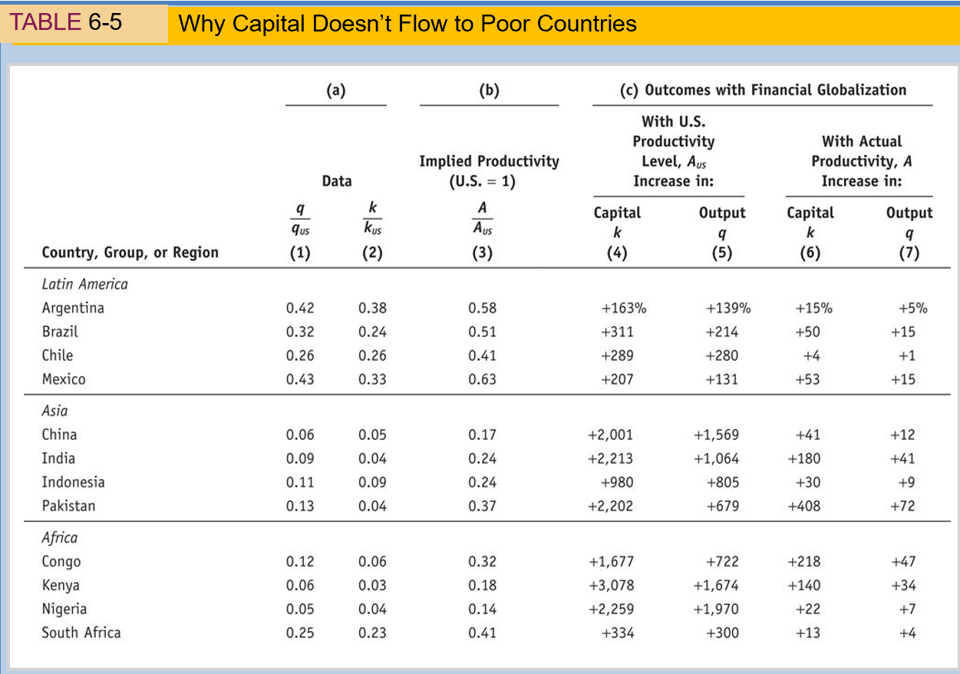
\includegraphics{pic3.png}
\end{frame}

\begin{frame}{A vs k}
\phantomsection\label{a-vs-k-2}
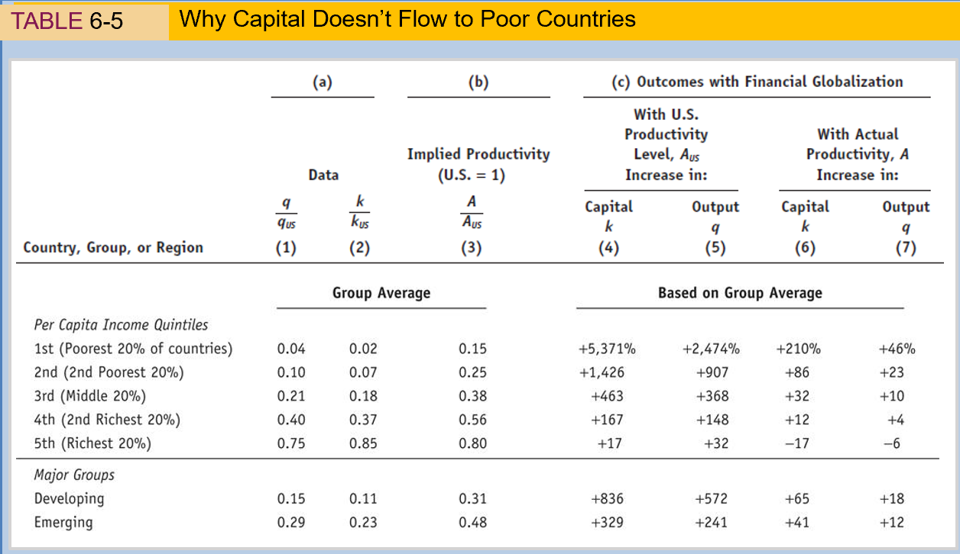
\includegraphics{pic4.png}
\end{frame}

\begin{frame}{A vs k}
\phantomsection\label{a-vs-k-3}
\begin{itemize}
\tightlist
\item
  An older school of thought focused on A as reflecting a country's
  technical efficiency, construed narrowly as a function of its
  technology and management capabilities.
\item
  Today, many economists believe that the level of A may primarily
  reflect a country's social efficiency, construed broadly to include
  institutions, public policies, and cultural differences.
\item
  And indeed there is some evidence that, among poorer countries,
  capital tends to flow to the countries with better institutions.
\end{itemize}
\end{frame}

\begin{frame}{A vs k}
\phantomsection\label{a-vs-k-4}
Other factors are against the likelihood of convergence.

\begin{itemize}
\tightlist
\item
  The model makes no allowance for risk premiums to compensate for the
  risk of investing in an emerging market (e.g., risks of regulatory
  changes, tax changes, expropriation, and other political risks).
\item
  Risk premiums can be substantial, and may be large enough to cause
  capital to flow ``uphill'' from poor to rich.
\end{itemize}
\end{frame}

\begin{frame}{A vs k}
\phantomsection\label{a-vs-k-5}
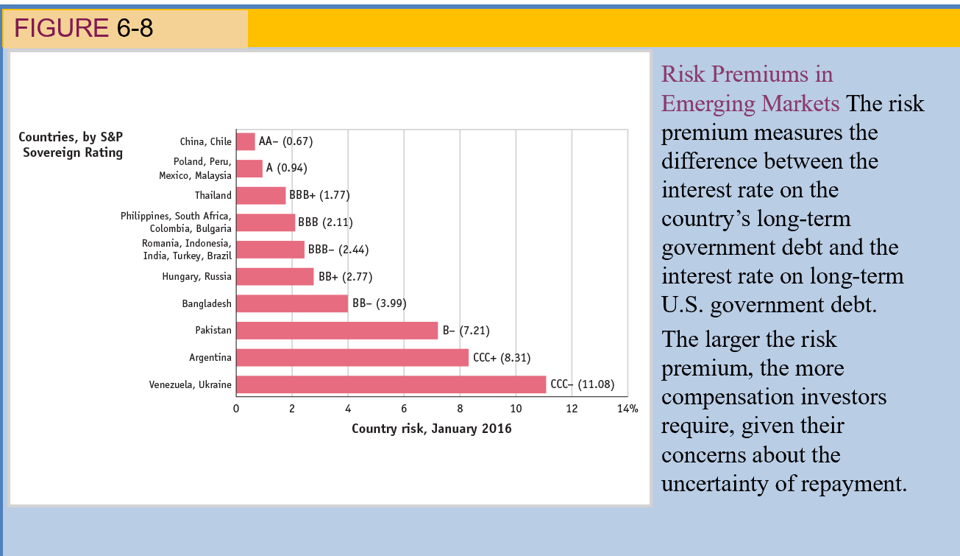
\includegraphics{pic5.png}
\end{frame}

\begin{frame}{A vs k}
\phantomsection\label{a-vs-k-6}
\begin{itemize}
\item
  The model assumes that investment goods can be acquired at the same
  relative price, but in developing countries, it often costs much more
  than one unit of output to purchase one unit of capital goods.
\item
  The model assumes that the contribution of capital to production is
  equal across countries, but the capital's share may be much lower in
  many developing countries. This lowers the MPK even more.
\end{itemize}
\end{frame}

\begin{frame}{A vs k}
\phantomsection\label{a-vs-k-7}
\begin{itemize}
\tightlist
\item
  The model suggests that foreign aid may do no better than foreign
  investors in promoting growth.
\item
  Economists dispute whether foreign aid can make a difference to
  long-term development and growth.
\item
  The argument also extends to nonmarket and preferential lending
  offered to poor countries by international financial institutions such
  as the World Bank.
\item
  Proponents argue that aid can finance public goods that can provide
  externalities sufficient to jolt a poor country out of a bad
  equilibrium or ``poverty trap.'' Aid skeptics reply that the evidence
  for such effects is weak.
\end{itemize}
\end{frame}

\begin{frame}{World bank}
\phantomsection\label{world-bank}
The World Bank (worldbank.org), based in Washington, D.C., is one of the
Bretton Woods ``twins'' established in 1944 (the other is the
International Monetary Fund).

Its main arm, the International Bank for Reconstruction and Development,
has 188 member countries. Its principal purpose is to provide financing
and technical assistance to reduce poverty and promote sustained
economic development in poor countries.

The World Bank can raise funds at low interest rates and issue AAA-rated
debt as good as that of any sovereign nation. It then lends to poor
borrowers at low rates.
\end{frame}

\begin{frame}{Foreign aid}
\phantomsection\label{foreign-aid}
Nobody doubts that vast amounts of aid have been squandered, but there
are reasons to think that we can improve on that record.

We now understand that the kind of aid you give, and the policies of the
countries you give it to, makes a real difference.

There's still a lot wrong with the way that foreign aid is administered.
Too little attention is paid to figuring out which programs work and
which don't, and aid still takes too little advantage of market
mechanisms, which are essential to making improvements last.
\end{frame}

\begin{frame}{Diversification of risk}
\phantomsection\label{diversification-of-risk}
Diversification can help smooth shocks by promoting risk sharing. With
diversification, countries may be able to reduce the volatility of their
incomes without any net lending or borrowing.

\begin{itemize}
\item
  We consider two countries, A and B, with outputs that fluctuate
  asymmetrically.
\item
  There are two possible ``states of the world,'' with equal probability
  of occurring. State 1 is a bad state for A and a good state for B;
  state 2 is good for A and bad for B.
\item
  We assume that all output is consumed, and that there is no investment
  or government spending. Output is divided 60--40 between labor income
  and capital income.
\end{itemize}
\end{frame}

\begin{frame}{Home portfolio}
\phantomsection\label{home-portfolio}
\begin{itemize}
\item
  Both countries are closed, and each owns 100\% of its capital. Output
  is the same as income.
\item
  A numerical example is given in Table 6-6, panel (a).
\item
  In state 1, A's output is 90, of which 54 units are payments to labor
  and 36 units are payments to capital; in state 2, A's output rises to
  110, and factor payments rise to 66 for labor and 44 units for
  capital. The opposite is true in B: In state 1, B's output is higher
  than it is in state 2.
\item
  The variation of GNI about its mean of 100 is plus or minus 10 in each
  country. Because households prefer smooth consumption, this variation
  is undesirable.
\end{itemize}
\end{frame}

\begin{frame}{Risk diversification}
\phantomsection\label{risk-diversification}
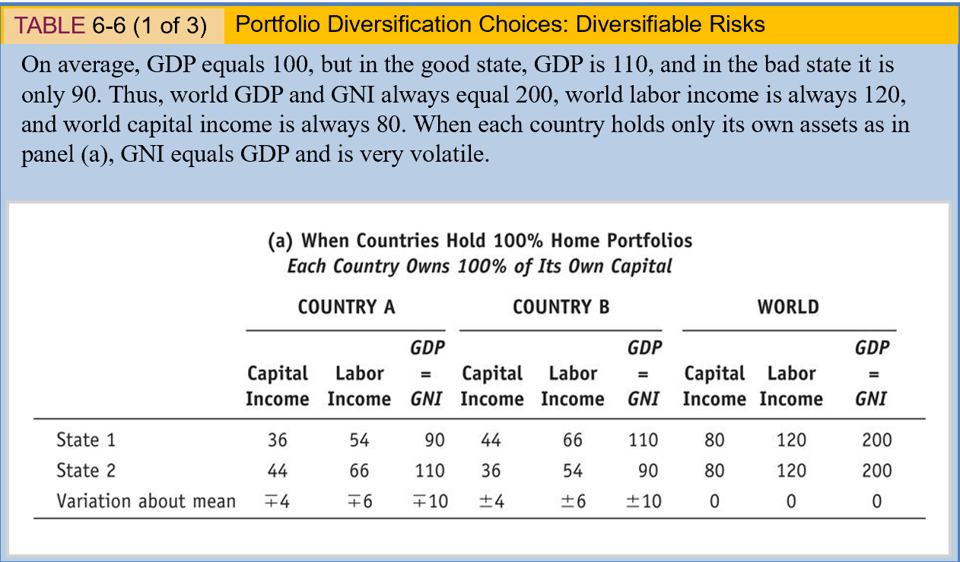
\includegraphics{pic5a.png}
\end{frame}

\begin{frame}{World Portfolio}
\phantomsection\label{world-portfolio}
\begin{itemize}
\item
  Two countries can achieve partial income smoothing if they diversify
  their portfolios of capital assets.
\item
  For example, each country could own half of the domestic capital
  stock, and half of the other country's capital stock. Indeed, this is
  what standard portfolio theory says that investors should try to do.
\item
  The results of this portfolio diversification are shown in Table 6-6,
  panel (b).
\item
  Capital income for each country is smoothed at 40 units, the average
  of A and B capital income in panel (a), also illustrated in Figure
  6-9.
\end{itemize}
\end{frame}

\begin{frame}{Risk diversification}
\phantomsection\label{risk-diversification-1}
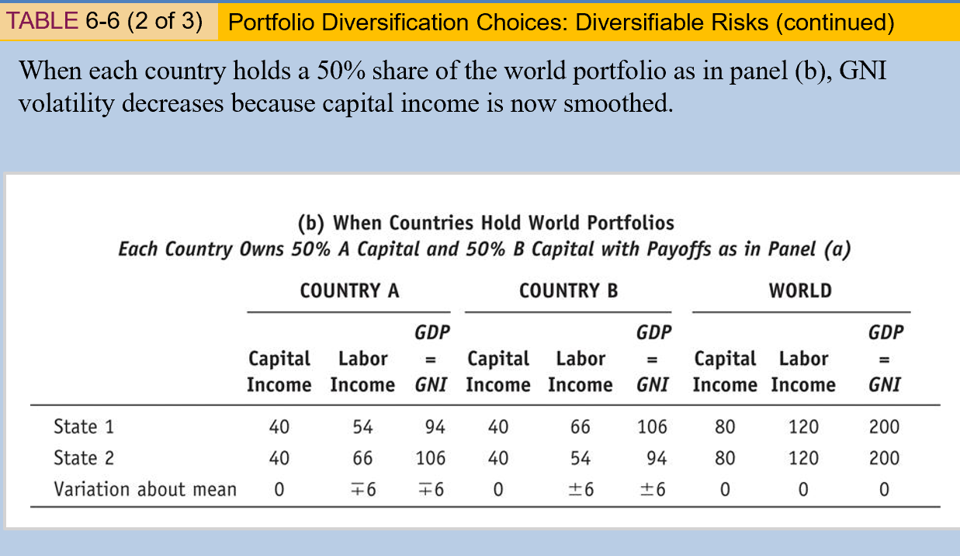
\includegraphics{pic6.png}
\end{frame}

\begin{frame}{Risk diversification}
\phantomsection\label{risk-diversification-2}
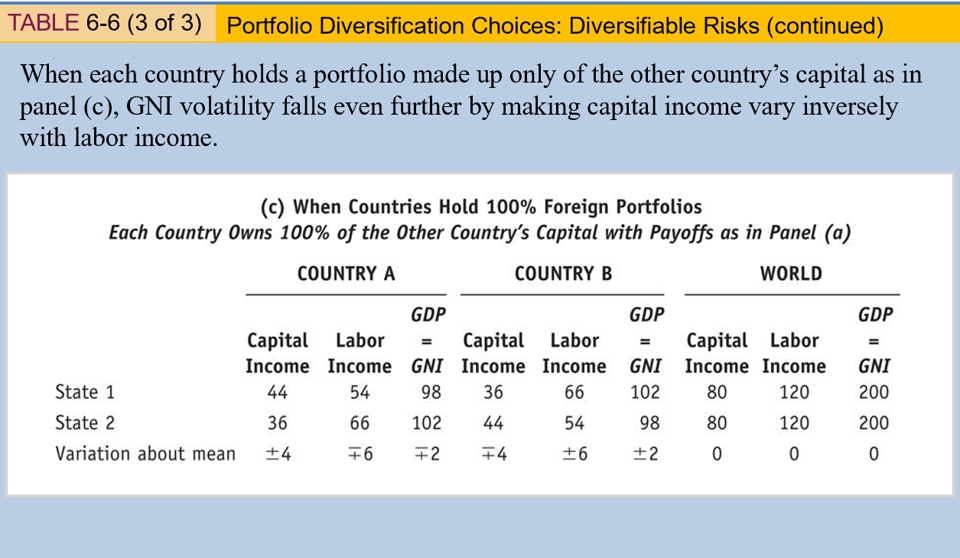
\includegraphics{pic7.png}
\end{frame}

\begin{frame}{Risk diversification}
\phantomsection\label{risk-diversification-3}
\begin{itemize}
\item
  How does the balance of payments work when countries hold the world
  portfolio?
\item
  Consider country A. In state 1 (bad for A, good for B), A's income or
  GNI exceeds A's output. The extra income is net factor income from
  abroad, which is the difference between the income earned on A's
  external assets and the income paid on A's external liabilities.
\item
  With that net factor income, country A runs a negative trade balance,
  which means that A can consume more than it produces.
\item
  Adding the trade balance of --4 to net factor income from abroad of +4
  means that the current account is 0, and there is still no need for
  any net borrowing or lending.
\end{itemize}
\end{frame}

\begin{frame}{Risk diversification}
\phantomsection\label{risk-diversification-4}
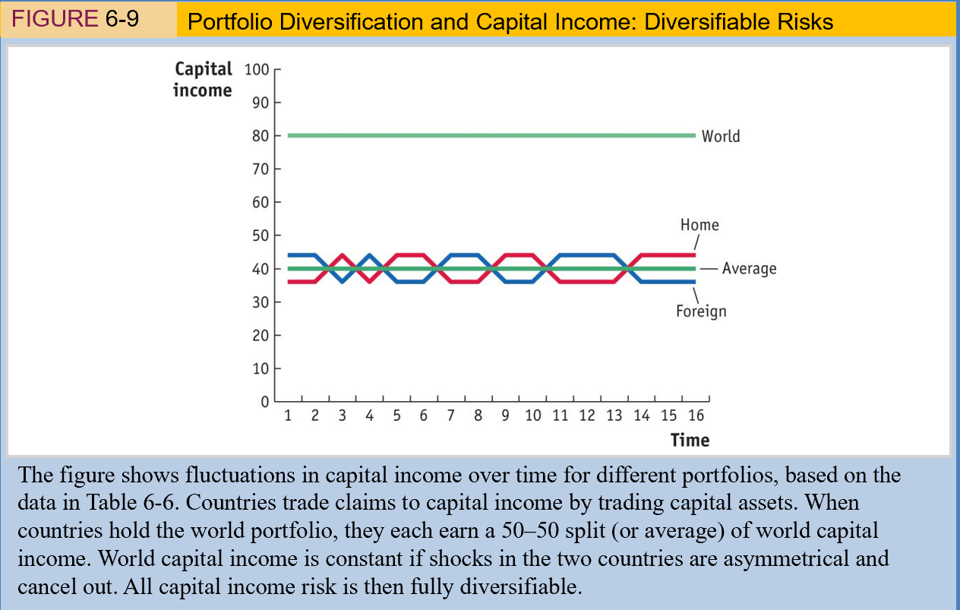
\includegraphics{pic8.png}
\end{frame}

\begin{frame}{Generalization}
\phantomsection\label{generalization}
Let us generalize the concept of capital income smoothing through
diversification.

\begin{itemize}
\item
  Each country's payments to capital are volatile. A portfolio of 100\%
  of country A's capital or 100\% of country B's capital has capital
  income that varies by plus or minus 4 (between 36 and 44). But a
  50--50 mix of the two leaves the investor with a portfolio of minimum,
  zero volatility (it always pays 40).
\item
  In general, there will be some common shocks, which are identical
  shocks experienced by both countries. In this case, there is no way to
  avoid this shock by portfolio diversification.
\item
  But as long as some shocks are asymmetric, the two countries can take
  advantage of gains from the diversification of risk.
\end{itemize}
\end{frame}

\begin{frame}{Generalization}
\phantomsection\label{generalization-1}
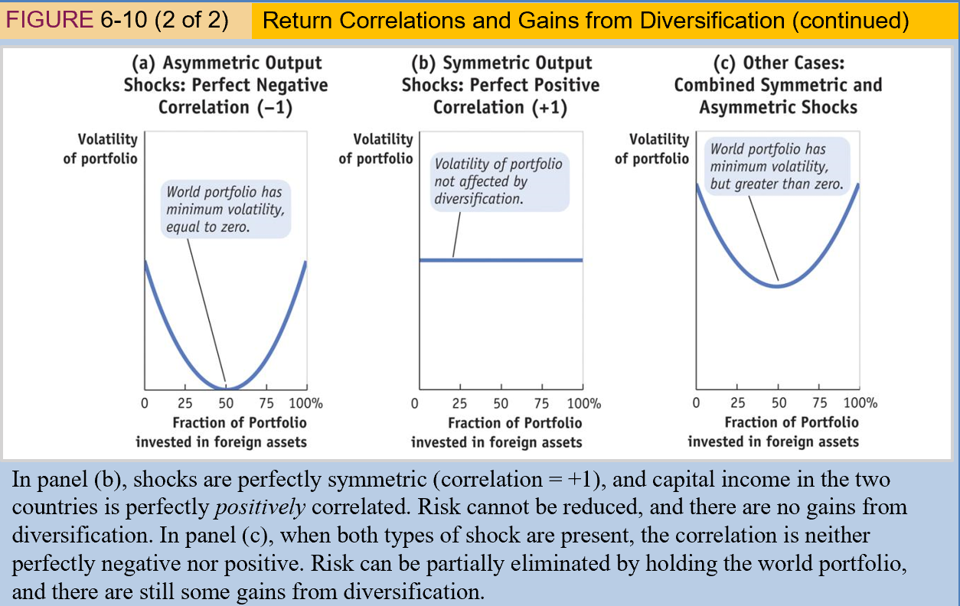
\includegraphics{pic9.png}
\end{frame}

\begin{frame}{Limits to Diversification}
\phantomsection\label{limits-to-diversification}
\begin{itemize}
\item
  Labor income risk (and hence GDP risk) may not be diversifiable
  through the trading of claims to labor assets or GDP.
\item
  But capital and labor income in each country are perfectly correlated,
  and shocks to production tend to raise and lower incomes of capital
  and labor simultaneously.
\item
  This means that, as a risk-sharing device, trading claims to capital
  income can substitute for trading claims to labor income.
\end{itemize}
\end{frame}

\begin{frame}{Home bias puzzle}
\phantomsection\label{home-bias-puzzle}
In practice, we do not observe countries owning foreign-biased
portfolios or even the world portfolio.

Countries tend to own portfolios that suffer from a strong home bias, a
tendency of investors to devote a disproportionate fraction of their
wealth to assets from their own home country, when a more globally
diversified portfolio might protect them better from risk.
\end{frame}

\begin{frame}{Diversification in US}
\phantomsection\label{diversification-in-us}
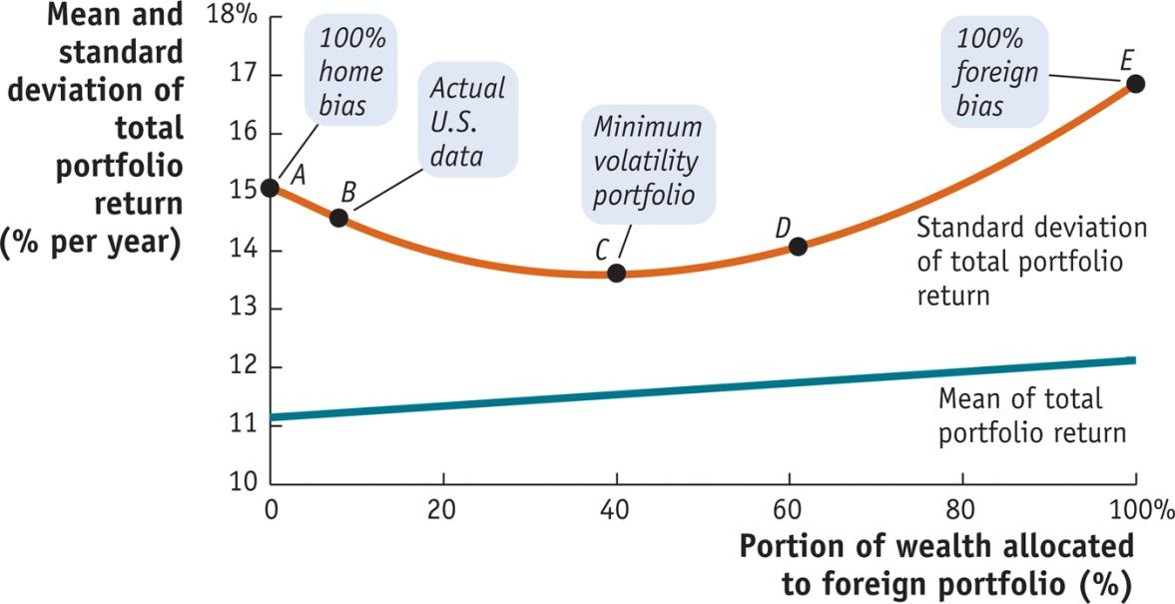
\includegraphics{pic10.jpg}
\end{frame}

\begin{frame}{Diversification in US}
\phantomsection\label{diversification-in-us-1}
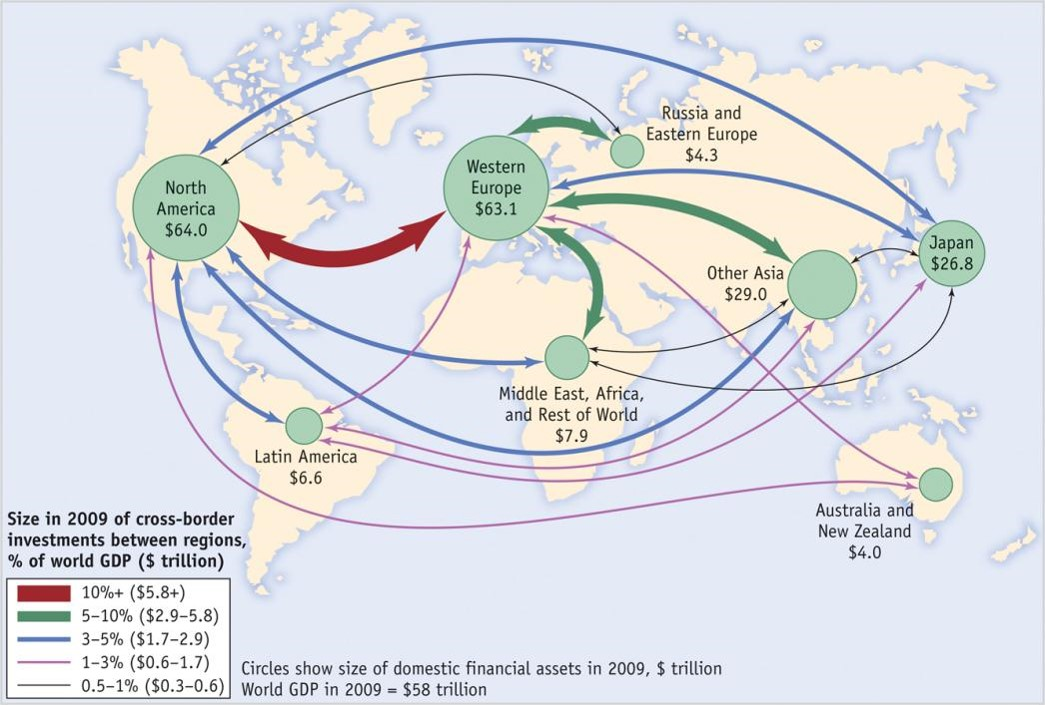
\includegraphics{pic11.jpg}
\end{frame}

\begin{frame}{Risk Diversification}
\phantomsection\label{risk-diversification-5}
If countries were able to borrow and lend without limit or restrictions,
they should be able to cope quite well with the array of possible
shocks, in order to smooth consumption.

\begin{itemize}
\item
  In reality, as the evidence shows, countries are not able to fully
  exploit the intertemporal borrowing mechanism.
\item
  In theory, if countries were able to pool their income streams and
  take shares from that common pool of income, all country-specific
  shocks would be averaged out, and the sole undiversifiable shocks
  would be common global shocks.
\end{itemize}
\end{frame}

\begin{frame}{Risk diversification}
\phantomsection\label{risk-diversification-6}
Financial openness allows countries---like households---to follow the
old adage ``Don't put all your eggs in one basket.''

\begin{itemize}
\item
  In practice, however, risk sharing through asset trade is limited. The
  market for claims to capital income is incomplete because not all
  capital assets are traded (e.g., many firms are privately held and are
  not listed on stock markets), and trade in labor assets is legally
  prohibited.
\item
  Investors have shown very little inclination to invest their wealth
  outside their own country, although that may be slowly changing in an
  environment of ongoing financial globalization.
\end{itemize}
\end{frame}

\begin{frame}{Conclusion}
\phantomsection\label{conclusion-1}
\begin{itemize}
\item
  Financial markets help households smooth consumption in the face of
  shocks to their income.
\item
  Financial markets allow firms to borrow in order to invest efficiently
  in productive projects and permit investors to diversify their
  portfolios across a wide range of assets.
\item
  The same principles apply to countries, subject to the long-run budget
  constraint. They face income shocks, new investment opportunities, and
  country-specific risks.
\item
  However, the use of global financial markets is still limited. Even in
  advanced countries, consumption shocks remain, investment is often
  financed out of domestic saving, and a home bias persists in
  investors' portfolios.
\end{itemize}
\end{frame}

\begin{frame}{Conclusion}
\phantomsection\label{conclusion-2}
\begin{itemize}
\item
  We see no consumption smoothing gains in poorer countries, and there
  is little scope for development based on external finance until
  productivity levels are improved.
\item
  Many emerging markets are still on the road to full financial
  liberalization, and large barriers remain.
\item
  Institutional weaknesses in developing countries may hinder the
  efficient operation of the mechanisms we have studied. Such weaknesses
  may be corrected by the stimulus to competition, transparency,
  accountability, and stability that financial openness may provide.
\item
  The benefits of financial globalization are likely to be much smaller
  for these countries, and they must also be weighed against potential
  offsetting costs, such as the risk of crises.
\end{itemize}
\end{frame}




\end{document}
